\documentclass[10pt]{article}
\usepackage{tikz}
\usetikzlibrary{shapes.misc}
\usepackage[margin=0cm]{geometry}
\pagestyle{empty}
\tikzstyle{every node}=[cross out, draw, red]

\begin{document}

\vspace*{\fill}
\begin{center}
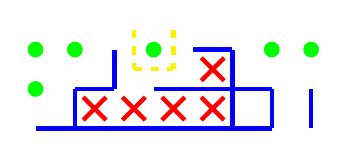
\begin{tikzpicture}[x=0.5cm, y=-0.5cm, ultra thick, blue]
% Walls
    \draw (4,0) -- (5,0);
    \draw (1,1) -- (2,1);
    \draw (3,1) -- (6,1);
    \draw (0,2) -- (6,2);
    \draw (1,1) -- (1,2);
    \draw (2,0) -- (2,1);
    \draw (5,0) -- (5,2);
    \draw (6,1) -- (6,2);
    \draw (7,1) -- (7,2);
% Pillars
    \fill[green] (0,0) circle(0.2);
    \fill[green] (1,0) circle(0.2);
    \fill[green] (3,0) circle(0.2);
    \fill[green] (6,0) circle(0.2);
    \fill[green] (7,0) circle(0.2);
    \fill[green] (0,1) circle(0.2);
% Inner points in accessible cul-de-sacs
    \node at (4.5,0.5) {};
    \node at (1.5,1.5) {};
    \node at (2.5,1.5) {};
    \node at (3.5,1.5) {};
    \node at (4.5,1.5) {};
% Entry-exit paths without intersections
    \draw[dashed, yellow] (2.5,0.5) -- (3.5,0.5);
    \draw[dashed, yellow] (2.5,-0.5) -- (2.5,0.5);
    \draw[dashed, yellow] (3.5,-0.5) -- (3.5,0.5);
\end{tikzpicture}
\end{center}
\vspace*{\fill}

\end{document}
